% !TEX root =  ../main_manuscript.tex 
\section{Results}
In PRIAS, the rate of reclassification within the first five years of follow-up was 35\%. This rate was capped at a maximum of 50\% in external GAP3 cohorts (Panel~B, Figure~\ref{fig:auc_beforecalib}). That is, many patients do not require any biopsy in the first five years. 

In the fitted joint model, when patient age increased from 61 to 71 years (25-th to 75-th percentile), the adjusted hazard ratio of reclassification was 1.45~(95\%CI:~1.30--1.63). When fitted PSA value (log scale) increased from 2.36 to 3.07 (25-th to 75-th percentile), the adjusted hazard ratio was 0.99~(95\%CI:~0.89--1.11). When estimated instantaneous PSA (log scale) velocity increased from -0.09 to 0.31 (25-th to 75-th percentile), the adjusted hazard ratio was 2.47~(95\%CI:~1.93--2.99). Hence, instantaneous velocity of PSA (log scale) was a stronger predictor for reclassification than its value. Detailed parameter estimates are in Supplementary~A.2.

The time-varying AUC and calibration of our model in different cohorts are shown in Panel~A and Panel~B of Figure~\ref{fig:auc_beforecalib}, respectively. The AUC achieves a moderate level in all cohorts. It fluctuates roughly around 0.63 over time. In terms of calibration, our model seems well calibrated only for the Johns Hopkins AS cohort. However, we resolved this issue by recalibrating the baseline hazard of our model separately for each cohort (Figure~6, Supplementary~B). The resulting risk predictions for individual patients from this recalibrated model and from separately fitted new joint models for each cohort were similar (Figure~7, Supplementary~B). Comprehensive discussion of validation results is in Supplementary~B.

\begin{figure}
\centerline{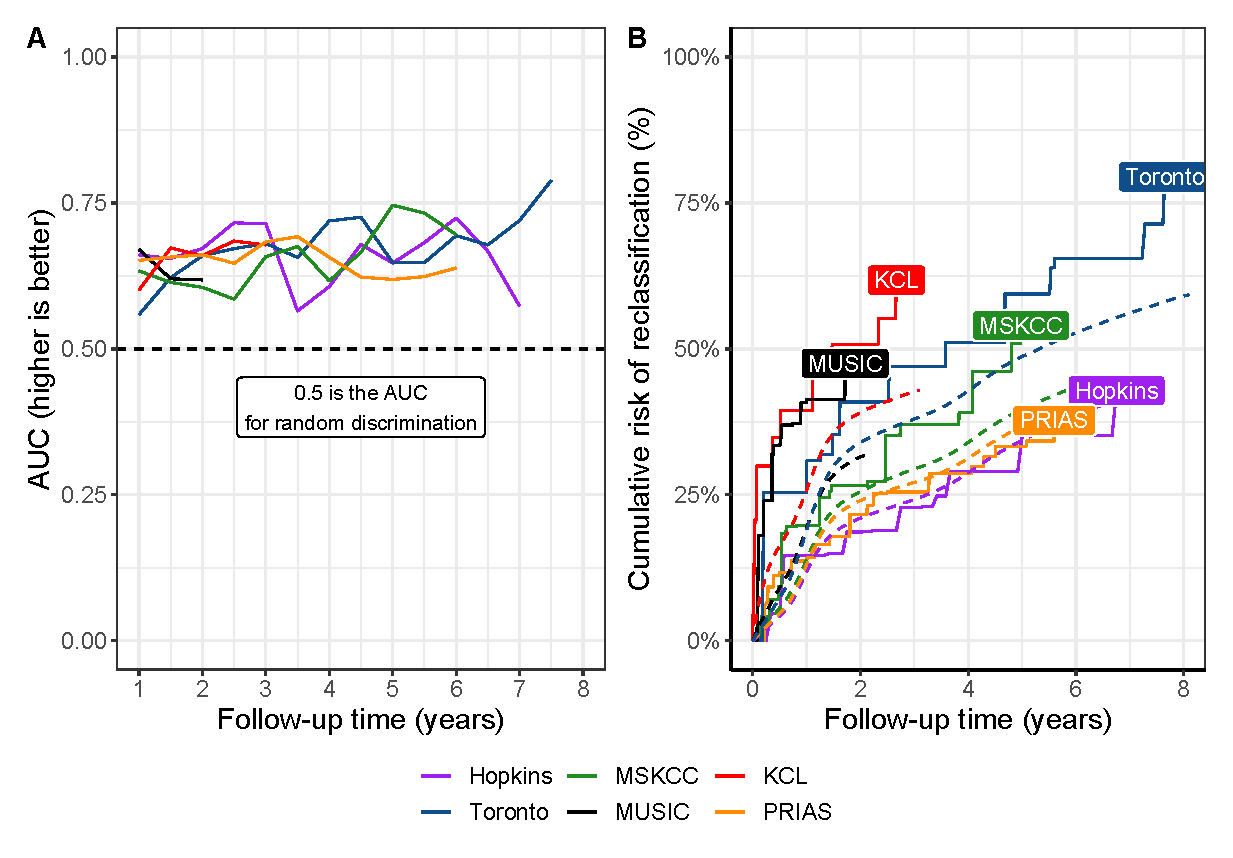
\includegraphics[width=\columnwidth]{images/auc_beforecalib.eps}}
\caption{\textbf{Model Validation Results}. \textbf{Panel~A}: time dependent area under the receiver operating characteristic curve or AUC (measure of discrimination). \textbf{Panel~B}: calibration-at-large~\citep{royston2013external,steyerberg2010assessing}, with solid lines depicting the non-parameteric estimate of the cumulative-risk of reclassification~\citep{turnbull1976empirical}, and dashed lines showing the average cumulative-risk of reclassification obtained using the joint model fitted to the PRIAS dataset. Full names of Cohorts are \textit{PRIAS}: Prostate Cancer International Active Surveillance, \textit{Toronto}: University of Toronto Active Surveillance, \textit{Hopkins}: Johns Hopkins Active Surveillance, \textit{MSKCC}: Memorial Sloan Kettering Cancer Center Active Surveillance, \textit{KCL}: King's College London Active Surveillance, \textit{MUSIC}: Michigan Urological Surgery Improvement Collaborative Active Surveillance.}
\label{fig:auc_beforecalib}
\end{figure}

Various personalized and fixed biopsy schedules for a demonstration patient in Figure~\ref{fig:demo_pat1} show that a personalized schedule based on 10\% risk threshold leads to one less biopsy than other schedules. At the same time, the corresponding time delay in detection of reclassification is expected to be only one month more than other schedules. A compulsory biopsy was scheduled at year six (maximum biopsy scheduling time of our model, Supplementary~C) in all schedules for a meaningful comparison across schedules. Schedules for other demonstration patients are in Figure~9--11, Supplementary~C.